% Options for packages loaded elsewhere
\PassOptionsToPackage{unicode}{hyperref}
\PassOptionsToPackage{hyphens}{url}
%
\documentclass[
]{article}
\usepackage{amsmath,amssymb}
\usepackage{lmodern}
\usepackage{iftex}
\ifPDFTeX
  \usepackage[T1]{fontenc}
  \usepackage[utf8]{inputenc}
  \usepackage{textcomp} % provide euro and other symbols
\else % if luatex or xetex
  \usepackage{unicode-math}
  \defaultfontfeatures{Scale=MatchLowercase}
  \defaultfontfeatures[\rmfamily]{Ligatures=TeX,Scale=1}
\fi
% Use upquote if available, for straight quotes in verbatim environments
\IfFileExists{upquote.sty}{\usepackage{upquote}}{}
\IfFileExists{microtype.sty}{% use microtype if available
  \usepackage[]{microtype}
  \UseMicrotypeSet[protrusion]{basicmath} % disable protrusion for tt fonts
}{}
\makeatletter
\@ifundefined{KOMAClassName}{% if non-KOMA class
  \IfFileExists{parskip.sty}{%
    \usepackage{parskip}
  }{% else
    \setlength{\parindent}{0pt}
    \setlength{\parskip}{6pt plus 2pt minus 1pt}}
}{% if KOMA class
  \KOMAoptions{parskip=half}}
\makeatother
\usepackage{xcolor}
\usepackage[margin=1in]{geometry}
\usepackage{color}
\usepackage{fancyvrb}
\newcommand{\VerbBar}{|}
\newcommand{\VERB}{\Verb[commandchars=\\\{\}]}
\DefineVerbatimEnvironment{Highlighting}{Verbatim}{commandchars=\\\{\}}
% Add ',fontsize=\small' for more characters per line
\usepackage{framed}
\definecolor{shadecolor}{RGB}{248,248,248}
\newenvironment{Shaded}{\begin{snugshade}}{\end{snugshade}}
\newcommand{\AlertTok}[1]{\textcolor[rgb]{0.94,0.16,0.16}{#1}}
\newcommand{\AnnotationTok}[1]{\textcolor[rgb]{0.56,0.35,0.01}{\textbf{\textit{#1}}}}
\newcommand{\AttributeTok}[1]{\textcolor[rgb]{0.77,0.63,0.00}{#1}}
\newcommand{\BaseNTok}[1]{\textcolor[rgb]{0.00,0.00,0.81}{#1}}
\newcommand{\BuiltInTok}[1]{#1}
\newcommand{\CharTok}[1]{\textcolor[rgb]{0.31,0.60,0.02}{#1}}
\newcommand{\CommentTok}[1]{\textcolor[rgb]{0.56,0.35,0.01}{\textit{#1}}}
\newcommand{\CommentVarTok}[1]{\textcolor[rgb]{0.56,0.35,0.01}{\textbf{\textit{#1}}}}
\newcommand{\ConstantTok}[1]{\textcolor[rgb]{0.00,0.00,0.00}{#1}}
\newcommand{\ControlFlowTok}[1]{\textcolor[rgb]{0.13,0.29,0.53}{\textbf{#1}}}
\newcommand{\DataTypeTok}[1]{\textcolor[rgb]{0.13,0.29,0.53}{#1}}
\newcommand{\DecValTok}[1]{\textcolor[rgb]{0.00,0.00,0.81}{#1}}
\newcommand{\DocumentationTok}[1]{\textcolor[rgb]{0.56,0.35,0.01}{\textbf{\textit{#1}}}}
\newcommand{\ErrorTok}[1]{\textcolor[rgb]{0.64,0.00,0.00}{\textbf{#1}}}
\newcommand{\ExtensionTok}[1]{#1}
\newcommand{\FloatTok}[1]{\textcolor[rgb]{0.00,0.00,0.81}{#1}}
\newcommand{\FunctionTok}[1]{\textcolor[rgb]{0.00,0.00,0.00}{#1}}
\newcommand{\ImportTok}[1]{#1}
\newcommand{\InformationTok}[1]{\textcolor[rgb]{0.56,0.35,0.01}{\textbf{\textit{#1}}}}
\newcommand{\KeywordTok}[1]{\textcolor[rgb]{0.13,0.29,0.53}{\textbf{#1}}}
\newcommand{\NormalTok}[1]{#1}
\newcommand{\OperatorTok}[1]{\textcolor[rgb]{0.81,0.36,0.00}{\textbf{#1}}}
\newcommand{\OtherTok}[1]{\textcolor[rgb]{0.56,0.35,0.01}{#1}}
\newcommand{\PreprocessorTok}[1]{\textcolor[rgb]{0.56,0.35,0.01}{\textit{#1}}}
\newcommand{\RegionMarkerTok}[1]{#1}
\newcommand{\SpecialCharTok}[1]{\textcolor[rgb]{0.00,0.00,0.00}{#1}}
\newcommand{\SpecialStringTok}[1]{\textcolor[rgb]{0.31,0.60,0.02}{#1}}
\newcommand{\StringTok}[1]{\textcolor[rgb]{0.31,0.60,0.02}{#1}}
\newcommand{\VariableTok}[1]{\textcolor[rgb]{0.00,0.00,0.00}{#1}}
\newcommand{\VerbatimStringTok}[1]{\textcolor[rgb]{0.31,0.60,0.02}{#1}}
\newcommand{\WarningTok}[1]{\textcolor[rgb]{0.56,0.35,0.01}{\textbf{\textit{#1}}}}
\usepackage{graphicx}
\makeatletter
\def\maxwidth{\ifdim\Gin@nat@width>\linewidth\linewidth\else\Gin@nat@width\fi}
\def\maxheight{\ifdim\Gin@nat@height>\textheight\textheight\else\Gin@nat@height\fi}
\makeatother
% Scale images if necessary, so that they will not overflow the page
% margins by default, and it is still possible to overwrite the defaults
% using explicit options in \includegraphics[width, height, ...]{}
\setkeys{Gin}{width=\maxwidth,height=\maxheight,keepaspectratio}
% Set default figure placement to htbp
\makeatletter
\def\fps@figure{htbp}
\makeatother
\setlength{\emergencystretch}{3em} % prevent overfull lines
\providecommand{\tightlist}{%
  \setlength{\itemsep}{0pt}\setlength{\parskip}{0pt}}
\setcounter{secnumdepth}{5}
\ifLuaTeX
  \usepackage{selnolig}  % disable illegal ligatures
\fi
\IfFileExists{bookmark.sty}{\usepackage{bookmark}}{\usepackage{hyperref}}
\IfFileExists{xurl.sty}{\usepackage{xurl}}{} % add URL line breaks if available
\urlstyle{same} % disable monospaced font for URLs
\hypersetup{
  pdftitle={HUDM6026 Homework\_10},
  pdfauthor={Chenguang Pan \& Seng Lei},
  hidelinks,
  pdfcreator={LaTeX via pandoc}}

\title{HUDM6026 Homework\_10}
\author{Chenguang Pan \& Seng Lei}
\date{April 04, 2023}

\begin{document}
\maketitle

\hypertarget{islr_chapter-6.10}{%
\subsection{ISLR\_Chapter 6.10}\label{islr_chapter-6.10}}

\emph{We have seen that as the number of features used in a model
increases, the training error will necessarily decrease, but the test
error may not. We will now explore this in a simulated data set.}

\hypertarget{a}{%
\subsubsection{(a)}\label{a}}

\emph{Generate a data set with p = 20 features, n = 1,000 observations,
and an associated quantitative response vector generated according to
the model}

\textbf{MY SOLUTION:}

Thinking multiple variate regression in matrix form provides a more
efficient way to estimate or simulate. Since generating the multivariate
normal distribution needs the connivance matrix and mean vector, like
shown in Dr.Keller's in-class R syntax, we need to define them first.

\begin{Shaded}
\begin{Highlighting}[]
\SpecialCharTok{\textgreater{}} \CommentTok{\# import the packages}
\ErrorTok{\textgreater{}} \FunctionTok{library}\NormalTok{(mvtnorm)}
\SpecialCharTok{\textgreater{}} \FunctionTok{library}\NormalTok{(clusterGeneration)}
\SpecialCharTok{\textgreater{}} 
\ErrorTok{\textgreater{}} \CommentTok{\# {-}{-}{-}{-}{-}{-}{-}{-}{-}{-}{-}{-}{-}{-}{-}{-}{-}{-}{-}{-}{-}}
\ErrorTok{\textgreater{}} \CommentTok{\# STAGE 1 PREPARE}
\ErrorTok{\textgreater{}} \CommentTok{\# {-}{-}{-}{-}{-}{-}{-}{-}{-}{-}{-}{-}{-}{-}{-}{-}{-}{-}{-}{-}{-}}
\ErrorTok{\textgreater{}} \CommentTok{\# set the random seed}
\ErrorTok{\textgreater{}} \FunctionTok{set.seed}\NormalTok{(}\DecValTok{666}\NormalTok{)}
\SpecialCharTok{\textgreater{}} \CommentTok{\# Generate a random covariance matrix with package clusterGeneration}
\ErrorTok{\textgreater{}}\NormalTok{ cov1 }\OtherTok{\textless{}{-}} \FunctionTok{genPositiveDefMat}\NormalTok{(}\AttributeTok{dim=}\DecValTok{20}\NormalTok{, }\CommentTok{\# create 20 covariates}
\SpecialCharTok{+}                           \AttributeTok{covMethod =} \StringTok{"eigen"}\NormalTok{)}
\SpecialCharTok{\textgreater{}} \CommentTok{\# Generate a random vector of 20 means from a normal distribution with N(0, 20)}
\ErrorTok{\textgreater{}}\NormalTok{ mns1 }\OtherTok{\textless{}{-}} \FunctionTok{rnorm}\NormalTok{(}\DecValTok{20}\NormalTok{,}\DecValTok{0}\NormalTok{,}\AttributeTok{sd=}\DecValTok{20}\NormalTok{)}
\SpecialCharTok{\textgreater{}} \CommentTok{\# Generate coefficients vector for the output for Y from norm(0, 1)  }
\ErrorTok{\textgreater{}}\NormalTok{ coef1 }\OtherTok{\textless{}{-}} \FunctionTok{rnorm}\NormalTok{(}\DecValTok{21}\NormalTok{, }\CommentTok{\# Beta0 + Beta1 +...+ Beta20}
\SpecialCharTok{+}                \DecValTok{0}\NormalTok{,}\DecValTok{1}\NormalTok{) }\CommentTok{\# drawn from a normal distribution N(0,1)}
\SpecialCharTok{\textgreater{}} \DocumentationTok{\#\#\# Set ten of them equal to zero}
\ErrorTok{\textgreater{}}\NormalTok{ coef1[}\FunctionTok{sample}\NormalTok{(}\DecValTok{2}\SpecialCharTok{:}\DecValTok{21}\NormalTok{, }\DecValTok{10}\NormalTok{, }\AttributeTok{replace =} \ConstantTok{FALSE}\NormalTok{)] }\OtherTok{\textless{}{-}} \DecValTok{0}
\SpecialCharTok{\textgreater{}} 
\ErrorTok{\textgreater{}} \CommentTok{\# {-}{-}{-}{-}{-}{-}{-}{-}{-}{-}{-}{-}{-}{-}{-}{-}{-}{-}{-}{-}{-}{-}{-}{-}{-}{-}{-}{-}{-}{-}{-}{-}{-}{-}{-}{-}{-}{-}{-}}
\ErrorTok{\textgreater{}} \CommentTok{\# STAGE 2 BUILD DATA GENERATING FUNCTION}
\ErrorTok{\textgreater{}} \CommentTok{\# {-}{-}{-}{-}{-}{-}{-}{-}{-}{-}{-}{-}{-}{-}{-}{-}{-}{-}{-}{-}{-}{-}{-}{-}{-}{-}{-}{-}{-}{-}{-}{-}{-}{-}{-}{-}{-}{-}{-}}
\ErrorTok{\textgreater{}}\NormalTok{ dataGen }\OtherTok{\textless{}{-}} \ControlFlowTok{function}\NormalTok{(N)\{}
\SpecialCharTok{+}   \CommentTok{\# Generate the X matrix }
\SpecialCharTok{+}\NormalTok{   X }\OtherTok{\textless{}{-}} \FunctionTok{rmvnorm}\NormalTok{(}\AttributeTok{n=}\NormalTok{N, }\AttributeTok{mean =}\NormalTok{ mns1,}\AttributeTok{sigma =}\NormalTok{ cov1}\SpecialCharTok{$}\NormalTok{Sigma)}
\SpecialCharTok{+}   \CommentTok{\# augmenting the X matrix}
\SpecialCharTok{+}\NormalTok{   X\_aug }\OtherTok{\textless{}{-}} \FunctionTok{cbind}\NormalTok{(}\DecValTok{1}\NormalTok{,X)}
\SpecialCharTok{+}   \CommentTok{\# create the output Y with error term vector following the N(0,1)}
\SpecialCharTok{+}\NormalTok{   Y }\OtherTok{\textless{}{-}}\NormalTok{ X\_aug }\SpecialCharTok{\%*\%}\NormalTok{ coef1 }\SpecialCharTok{+} \FunctionTok{rnorm}\NormalTok{(N,}\DecValTok{0}\NormalTok{,}\DecValTok{1}\NormalTok{)}
\SpecialCharTok{+}   \CommentTok{\# adjust the output}
\SpecialCharTok{+}\NormalTok{   dfOut }\OtherTok{\textless{}{-}}  \FunctionTok{data.frame}\NormalTok{(}\FunctionTok{cbind}\NormalTok{(X,Y))}
\SpecialCharTok{+}   \FunctionTok{names}\NormalTok{(dfOut) }\OtherTok{\textless{}{-}} \FunctionTok{c}\NormalTok{(}\FunctionTok{paste0}\NormalTok{(}\StringTok{"X"}\NormalTok{,}\DecValTok{1}\SpecialCharTok{:}\DecValTok{20}\NormalTok{), }\StringTok{"Y"}\NormalTok{)}
\SpecialCharTok{+}   \FunctionTok{return}\NormalTok{(dfOut)}
\SpecialCharTok{+}\NormalTok{ \}}
\SpecialCharTok{\textgreater{}} 
\ErrorTok{\textgreater{}} \CommentTok{\# {-}{-}{-}{-}{-}{-}{-}{-}{-}{-}{-}{-}{-}{-}{-}{-}{-}{-}{-}{-}{-}{-}}
\ErrorTok{\textgreater{}} \CommentTok{\# STAGE 3 GENERATE DATA}
\ErrorTok{\textgreater{}} \CommentTok{\# {-}{-}{-}{-}{-}{-}{-}{-}{-}{-}{-}{-}{-}{-}{-}{-}{-}{-}{-}{-}{-}{-}}
\ErrorTok{\textgreater{}}\NormalTok{ df }\OtherTok{\textless{}{-}} \FunctionTok{dataGen}\NormalTok{(}\DecValTok{1000}\NormalTok{)}
\SpecialCharTok{\textgreater{}} \FunctionTok{head}\NormalTok{(df)}
\NormalTok{          X1        X2       X3        X4        X5        X6        X7}
\DecValTok{1} \SpecialCharTok{{-}}\FloatTok{15.654375} \SpecialCharTok{{-}}\FloatTok{23.63880} \FloatTok{23.30226} \SpecialCharTok{{-}}\FloatTok{9.037281}  \FloatTok{1.333409} \SpecialCharTok{{-}}\FloatTok{33.06151} \SpecialCharTok{{-}}\FloatTok{26.56916}
\DecValTok{2} \SpecialCharTok{{-}}\FloatTok{13.886764} \SpecialCharTok{{-}}\FloatTok{21.96735} \FloatTok{27.40210} \SpecialCharTok{{-}}\FloatTok{8.405507} \SpecialCharTok{{-}}\FloatTok{1.067594} \SpecialCharTok{{-}}\FloatTok{30.14542} \SpecialCharTok{{-}}\FloatTok{21.91764}
\DecValTok{3} \SpecialCharTok{{-}}\FloatTok{16.544472} \SpecialCharTok{{-}}\FloatTok{24.79274} \FloatTok{25.22519} \SpecialCharTok{{-}}\FloatTok{5.824548}  \FloatTok{2.412756} \SpecialCharTok{{-}}\FloatTok{32.54058} \SpecialCharTok{{-}}\FloatTok{24.17569}
\DecValTok{4} \SpecialCharTok{{-}}\FloatTok{12.779982} \SpecialCharTok{{-}}\FloatTok{20.92270} \FloatTok{21.60266} \SpecialCharTok{{-}}\FloatTok{6.448326} \SpecialCharTok{{-}}\FloatTok{2.055508} \SpecialCharTok{{-}}\FloatTok{28.52098} \SpecialCharTok{{-}}\FloatTok{20.26761}
\DecValTok{5}  \SpecialCharTok{{-}}\FloatTok{9.483628} \SpecialCharTok{{-}}\FloatTok{21.20340} \FloatTok{27.07318} \SpecialCharTok{{-}}\FloatTok{8.032887}  \FloatTok{1.118195} \SpecialCharTok{{-}}\FloatTok{26.48337} \SpecialCharTok{{-}}\FloatTok{18.48465}
\DecValTok{6}  \SpecialCharTok{{-}}\FloatTok{9.034796} \SpecialCharTok{{-}}\FloatTok{26.44232} \FloatTok{24.74899} \SpecialCharTok{{-}}\FloatTok{6.218634}  \FloatTok{1.071316} \SpecialCharTok{{-}}\FloatTok{32.66566} \SpecialCharTok{{-}}\FloatTok{23.47574}
\NormalTok{         X8        X9       X10      X11       X12      X13       X14      X15}
\DecValTok{1} \SpecialCharTok{{-}}\FloatTok{38.65066} \SpecialCharTok{{-}}\FloatTok{22.00314} \SpecialCharTok{{-}}\FloatTok{26.93117} \FloatTok{16.61306} \SpecialCharTok{{-}}\FloatTok{14.18094} \FloatTok{26.11095} \SpecialCharTok{{-}}\FloatTok{14.44719} \FloatTok{5.456897}
\DecValTok{2} \SpecialCharTok{{-}}\FloatTok{34.84637} \SpecialCharTok{{-}}\FloatTok{20.95672} \SpecialCharTok{{-}}\FloatTok{29.48340} \FloatTok{12.95538} \SpecialCharTok{{-}}\FloatTok{13.58884} \FloatTok{29.53441} \SpecialCharTok{{-}}\FloatTok{13.16991} \FloatTok{3.997159}
\DecValTok{3} \SpecialCharTok{{-}}\FloatTok{36.27806} \SpecialCharTok{{-}}\FloatTok{22.09635} \SpecialCharTok{{-}}\FloatTok{24.52454} \FloatTok{16.02539} \SpecialCharTok{{-}}\FloatTok{12.39565} \FloatTok{28.99292} \SpecialCharTok{{-}}\FloatTok{11.51038} \FloatTok{5.682973}
\DecValTok{4} \SpecialCharTok{{-}}\FloatTok{32.40778} \SpecialCharTok{{-}}\FloatTok{21.28272} \SpecialCharTok{{-}}\FloatTok{24.59206} \FloatTok{17.65221} \SpecialCharTok{{-}}\FloatTok{13.14092} \FloatTok{30.28706} \SpecialCharTok{{-}}\FloatTok{12.10753} \FloatTok{7.614404}
\DecValTok{5} \SpecialCharTok{{-}}\FloatTok{34.09399} \SpecialCharTok{{-}}\FloatTok{20.28110} \SpecialCharTok{{-}}\FloatTok{24.05303} \FloatTok{14.96859} \SpecialCharTok{{-}}\FloatTok{11.37569} \FloatTok{33.35054} \SpecialCharTok{{-}}\FloatTok{11.67114} \FloatTok{6.937878}
\DecValTok{6} \SpecialCharTok{{-}}\FloatTok{37.49877} \SpecialCharTok{{-}}\FloatTok{20.05385} \SpecialCharTok{{-}}\FloatTok{25.27227} \FloatTok{18.48872} \SpecialCharTok{{-}}\FloatTok{14.45867} \FloatTok{28.59119} \SpecialCharTok{{-}}\FloatTok{10.64753} \FloatTok{3.655086}
\NormalTok{       X16      X17       X18      X19      X20         Y}
\DecValTok{1} \FloatTok{9.945809} \FloatTok{7.827704} \SpecialCharTok{{-}}\FloatTok{27.34912} \FloatTok{4.186049} \FloatTok{39.31443} \SpecialCharTok{{-}}\FloatTok{60.59024}
\DecValTok{2} \FloatTok{6.217472} \FloatTok{8.767564} \SpecialCharTok{{-}}\FloatTok{30.60701} \FloatTok{4.419715} \FloatTok{43.42606} \SpecialCharTok{{-}}\FloatTok{65.44828}
\DecValTok{3} \FloatTok{7.294496} \FloatTok{9.247503} \SpecialCharTok{{-}}\FloatTok{28.08444} \FloatTok{7.811671} \FloatTok{45.24822} \SpecialCharTok{{-}}\FloatTok{62.32994}
\DecValTok{4} \FloatTok{7.385289} \FloatTok{8.772892} \SpecialCharTok{{-}}\FloatTok{30.73892} \FloatTok{2.614271} \FloatTok{40.79408} \SpecialCharTok{{-}}\FloatTok{65.53384}
\DecValTok{5} \FloatTok{3.612012} \FloatTok{9.087225} \SpecialCharTok{{-}}\FloatTok{26.15211} \FloatTok{5.705587} \FloatTok{42.05414} \SpecialCharTok{{-}}\FloatTok{66.31407}
\DecValTok{6} \FloatTok{4.453720} \FloatTok{9.404593} \SpecialCharTok{{-}}\FloatTok{29.21027} \FloatTok{5.087559} \FloatTok{42.82547} \SpecialCharTok{{-}}\FloatTok{63.94680}
\SpecialCharTok{\textgreater{}} \FunctionTok{dim}\NormalTok{(df)}
\NormalTok{[}\DecValTok{1}\NormalTok{] }\DecValTok{1000}   \DecValTok{21}
\end{Highlighting}
\end{Shaded}

The data looks good.

\hypertarget{b}{%
\subsubsection{(b)}\label{b}}

\emph{Split your dataset into a training set containing 100 observations
and a test set containing 900 observations.}

\textbf{MY SOLUTION:}

\begin{Shaded}
\begin{Highlighting}[]
\SpecialCharTok{\textgreater{}} \CommentTok{\# generate a random index from 1:1000 }
\ErrorTok{\textgreater{}} \FunctionTok{set.seed}\NormalTok{(}\DecValTok{666}\NormalTok{)}
\SpecialCharTok{\textgreater{}}\NormalTok{ index\_rdm }\OtherTok{\textless{}{-}} \FunctionTok{sample}\NormalTok{(}\FunctionTok{c}\NormalTok{(}\DecValTok{1}\SpecialCharTok{:}\DecValTok{1000}\NormalTok{),}\DecValTok{100}\NormalTok{)}
\SpecialCharTok{\textgreater{}} \CommentTok{\# separate the dataset into train and test dataset}
\ErrorTok{\textgreater{}}\NormalTok{ df\_train }\OtherTok{\textless{}{-}}\NormalTok{ df[index\_rdm,]}
\SpecialCharTok{\textgreater{}}\NormalTok{ df\_test }\OtherTok{\textless{}{-}}\NormalTok{ df[}\SpecialCharTok{{-}}\NormalTok{index\_rdm,]}
\SpecialCharTok{\textgreater{}} \FunctionTok{dim}\NormalTok{(df\_train)}
\NormalTok{[}\DecValTok{1}\NormalTok{] }\DecValTok{100}  \DecValTok{21}
\SpecialCharTok{\textgreater{}} \FunctionTok{dim}\NormalTok{(df\_test)}
\NormalTok{[}\DecValTok{1}\NormalTok{] }\DecValTok{900}  \DecValTok{21}
\end{Highlighting}
\end{Shaded}

The randomly-subseted train- and test-dataset look good.

\hypertarget{c}{%
\subsubsection{(c)}\label{c}}

\emph{Perform best subset selection on the training set, and plot the
training set MSE associated with the best model of each size.}

\textbf{MY SOLUTION:}

\begin{Shaded}
\begin{Highlighting}[]
\SpecialCharTok{\textgreater{}} \FunctionTok{library}\NormalTok{(bestglm)}
\SpecialCharTok{\textgreater{}}\NormalTok{ bss\_out }\OtherTok{\textless{}{-}} \FunctionTok{regsubsets}\NormalTok{(Y }\SpecialCharTok{\textasciitilde{}}\NormalTok{., }\AttributeTok{data =}\NormalTok{ df\_train, }\AttributeTok{nvmax=}\DecValTok{20}\NormalTok{)}
\SpecialCharTok{\textgreater{}}\NormalTok{ bss\_out\_summary }\OtherTok{\textless{}{-}} \FunctionTok{summary}\NormalTok{(bss\_out)}
\end{Highlighting}
\end{Shaded}

Note, by default, the \texttt{regsubsets()} only returns the first 8
models.\\
Based on the definition, we can get easily get the MSE since
\(MSE = \frac{RSS}{n}\).

\begin{Shaded}
\begin{Highlighting}[]
\SpecialCharTok{\textgreater{}} \FunctionTok{plot}\NormalTok{(bss\_out\_summary}\SpecialCharTok{$}\NormalTok{rss}\SpecialCharTok{/}\FunctionTok{nrow}\NormalTok{(df\_train),}
\SpecialCharTok{+}      \AttributeTok{xlab =} \StringTok{"Number of Vairables"}\NormalTok{,}
\SpecialCharTok{+}      \AttributeTok{ylab =} \StringTok{"MSE"}\NormalTok{,}
\SpecialCharTok{+}      \AttributeTok{type =} \StringTok{"l"}\NormalTok{)}
\SpecialCharTok{\textgreater{}} \FunctionTok{title}\NormalTok{(}\AttributeTok{main =} \StringTok{"Figure 1. Training set MSE associated with the best model of each size."}\NormalTok{, }
\SpecialCharTok{+}       \AttributeTok{cex.main =} \DecValTok{1}\NormalTok{)}
\end{Highlighting}
\end{Shaded}

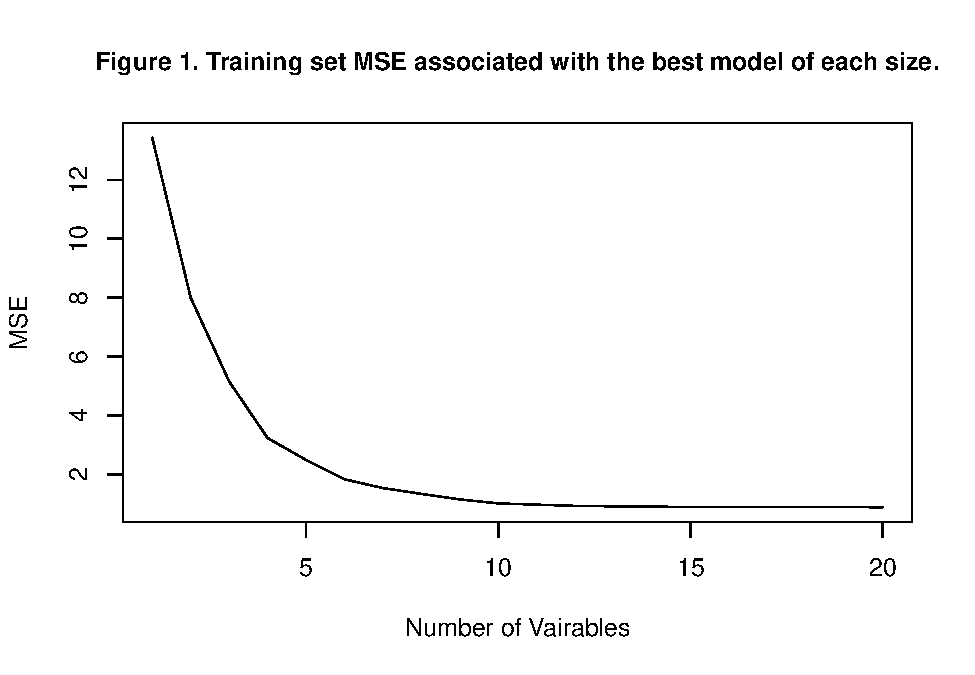
\includegraphics[width=0.5\linewidth,height=0.5\textheight]{Homework_10_Pan_files/figure-latex/unnamed-chunk-4-1}

\hypertarget{d}{%
\subsubsection{(d)}\label{d}}

\emph{Plot the test set MSE associated with the best model of each
size.}

\textbf{MY SOLUTION:}\\
Since there is no \texttt{predict()} function built in the
\texttt{regsubsets()}, I need to write by hand.

\begin{Shaded}
\begin{Highlighting}[]
\SpecialCharTok{\textgreater{}} \CommentTok{\# note the test dataset is in data.frame format need to be change to matrix}
\ErrorTok{\textgreater{}}\NormalTok{ df\_test\_matrix }\OtherTok{\textless{}{-}} \FunctionTok{as.matrix}\NormalTok{(df\_test)}
\SpecialCharTok{\textgreater{}} \FunctionTok{names}\NormalTok{(}\FunctionTok{coef}\NormalTok{(bss\_out, }\AttributeTok{id=}\DecValTok{2}\NormalTok{))[}\SpecialCharTok{{-}}\DecValTok{1}\NormalTok{]}
\NormalTok{[}\DecValTok{1}\NormalTok{] }\StringTok{"X19"} \StringTok{"X20"}
\SpecialCharTok{\textgreater{}} 
\ErrorTok{\textgreater{}}\NormalTok{ test\_mse }\OtherTok{\textless{}{-}} \FunctionTok{c}\NormalTok{()}
\SpecialCharTok{\textgreater{}} \ControlFlowTok{for}\NormalTok{ (i }\ControlFlowTok{in} \DecValTok{1}\SpecialCharTok{:}\DecValTok{20}\NormalTok{) \{}
\SpecialCharTok{+}   \CommentTok{\# to extract the coefficient vector for each best model}
\SpecialCharTok{+}\NormalTok{   coefi }\OtherTok{\textless{}{-}} \FunctionTok{coef}\NormalTok{(bss\_out, }\AttributeTok{id=}\NormalTok{i)}
\SpecialCharTok{+}   \CommentTok{\# select the corresponding variables and times the coefficients}
\SpecialCharTok{+}\NormalTok{   X\_temp }\OtherTok{\textless{}{-}}\NormalTok{ df\_test\_matrix[,}\FunctionTok{names}\NormalTok{(coefi)[}\SpecialCharTok{{-}}\DecValTok{1}\NormalTok{]]}
\SpecialCharTok{+}\NormalTok{   X\_temp\_aug }\OtherTok{\textless{}{-}} \FunctionTok{cbind}\NormalTok{(}\DecValTok{1}\NormalTok{, X\_temp)}
\SpecialCharTok{+}\NormalTok{   pred }\OtherTok{\textless{}{-}}\NormalTok{ X\_temp\_aug }\SpecialCharTok{\%*\%}\NormalTok{ coefi}
\SpecialCharTok{+}   \CommentTok{\# use the estimated vector of outcome to get the MSE}
\SpecialCharTok{+}\NormalTok{   mse }\OtherTok{\textless{}{-}} \FunctionTok{mean}\NormalTok{((df\_test[,}\StringTok{"Y"}\NormalTok{]}\SpecialCharTok{{-}}\NormalTok{pred)}\SpecialCharTok{\^{}}\DecValTok{2}\NormalTok{)}
\SpecialCharTok{+}\NormalTok{   test\_mse[i] }\OtherTok{\textless{}{-}}\NormalTok{ mse}
\SpecialCharTok{+}\NormalTok{ \}}
\SpecialCharTok{\textgreater{}}\NormalTok{ test\_mse}
\NormalTok{ [}\DecValTok{1}\NormalTok{] }\FloatTok{14.587205}  \FloatTok{7.695202}  \FloatTok{4.852660}  \FloatTok{3.615263}  \FloatTok{2.790152}  \FloatTok{1.987071}  \FloatTok{1.975713}
\NormalTok{ [}\DecValTok{8}\NormalTok{]  }\FloatTok{1.442175}  \FloatTok{1.207953}  \FloatTok{1.073172}  \FloatTok{1.151072}  \FloatTok{1.257745}  \FloatTok{1.295256}  \FloatTok{1.316578}
\NormalTok{[}\DecValTok{15}\NormalTok{]  }\FloatTok{1.350052}  \FloatTok{1.343764}  \FloatTok{1.340008}  \FloatTok{1.357865}  \FloatTok{1.362500}  \FloatTok{1.356349}
\end{Highlighting}
\end{Shaded}

The result looks good. Next, I plot the MSE.

\begin{Shaded}
\begin{Highlighting}[]
\SpecialCharTok{\textgreater{}} \FunctionTok{plot}\NormalTok{(test\_mse,}
\SpecialCharTok{+}      \AttributeTok{xlab =} \StringTok{"Number of Vairables"}\NormalTok{,}
\SpecialCharTok{+}      \AttributeTok{ylab =} \StringTok{"MSE"}\NormalTok{,}
\SpecialCharTok{+}      \AttributeTok{type =} \StringTok{"l"}\NormalTok{)}
\SpecialCharTok{\textgreater{}} \FunctionTok{title}\NormalTok{(}\AttributeTok{main =} \StringTok{"Figure 2. Test{-}set MSE associated with the best model of each size."}\NormalTok{, }
\SpecialCharTok{+}       \AttributeTok{cex.main =} \DecValTok{1}\NormalTok{)}
\SpecialCharTok{\textgreater{}}\NormalTok{ min\_index }\OtherTok{\textless{}{-}} \FunctionTok{which.min}\NormalTok{(test\_mse)}
\SpecialCharTok{\textgreater{}} \FunctionTok{points}\NormalTok{(min\_index,test\_mse[min\_index],}\AttributeTok{col=}\StringTok{"red"}\NormalTok{,}\AttributeTok{cex=}\DecValTok{2}\NormalTok{, }\AttributeTok{pch=}\DecValTok{20}\NormalTok{)}
\SpecialCharTok{\textgreater{}} \FunctionTok{abline}\NormalTok{(}\AttributeTok{h=}\FunctionTok{min}\NormalTok{(test\_mse), }\AttributeTok{col=}\StringTok{"red"}\NormalTok{,}\AttributeTok{lty=}\StringTok{"longdash"}\NormalTok{)}
\end{Highlighting}
\end{Shaded}

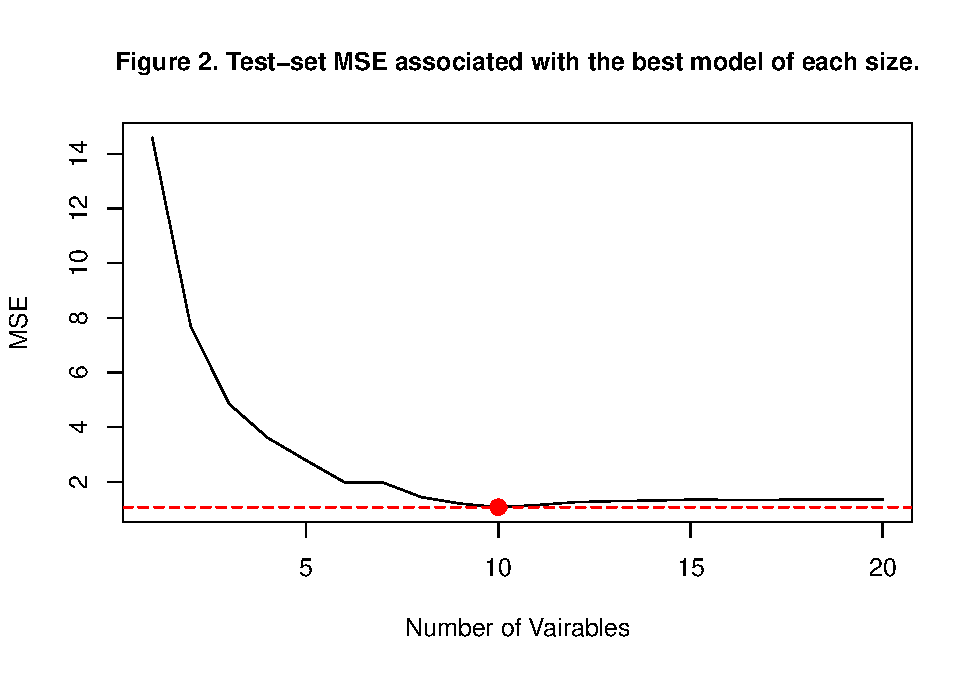
\includegraphics[width=0.5\linewidth,height=0.5\textheight]{Homework_10_Pan_files/figure-latex/unnamed-chunk-6-1}

\hypertarget{e}{%
\subsubsection{(e)}\label{e}}

\emph{For which model size does the test set MSE take on its minimum
value? Comment on your results.}

\textbf{MY SOLUTION:}\\
\emph{Figure 2} shows that the model with 10 predictors has the lowest
test MSE. From the results below, the ten covariates are
\(X1\),\(X4\),\(X7\),\(X9\),\(X10\),\(X13\),\(X14\),\(X15\),\(X19\), and
\(X20\).

\begin{Shaded}
\begin{Highlighting}[]
\SpecialCharTok{\textgreater{}}\NormalTok{ bss\_out\_summary}\SpecialCharTok{$}\NormalTok{outmat[}\DecValTok{10}\NormalTok{,]}
\NormalTok{ X1  X2  X3  X4  X5  X6  X7  X8  X9 X10 X11 X12 X13 X14 X15 X16 X17 X18 X19 X20 }
\StringTok{"*"} \StringTok{" "} \StringTok{" "} \StringTok{"*"} \StringTok{" "} \StringTok{" "} \StringTok{"*"} \StringTok{" "} \StringTok{"*"} \StringTok{"*"} \StringTok{" "} \StringTok{" "} \StringTok{"*"} \StringTok{"*"} \StringTok{"*"} \StringTok{" "} \StringTok{" "} \StringTok{" "} \StringTok{"*"} \StringTok{"*"} 
\end{Highlighting}
\end{Shaded}

\hypertarget{f}{%
\subsubsection{(f)}\label{f}}

\emph{How does the model at which the test set MSE is minimized compare
to the true model used to generate the data? }

\textbf{MY SOLUTION:}

\begin{Shaded}
\begin{Highlighting}[]
\SpecialCharTok{\textgreater{}} \CommentTok{\# extract the estimated 10{-}predictor model\textquotesingle{}s coefficient}
\ErrorTok{\textgreater{}} \FunctionTok{round}\NormalTok{(}\FunctionTok{coef}\NormalTok{(bss\_out,}\AttributeTok{id=}\DecValTok{10}\NormalTok{),}\DecValTok{3}\NormalTok{)}
\NormalTok{(Intercept)          X1          X4          X7          X9         X10 }
      \FloatTok{9.692}      \SpecialCharTok{{-}}\FloatTok{0.448}       \FloatTok{0.486}       \FloatTok{0.146}       \FloatTok{0.391}       \FloatTok{0.213} 
\NormalTok{        X13         X14         X15         X19         X20 }
     \SpecialCharTok{{-}}\FloatTok{0.748}      \SpecialCharTok{{-}}\FloatTok{0.353}      \SpecialCharTok{{-}}\FloatTok{0.785}       \FloatTok{1.306}      \SpecialCharTok{{-}}\FloatTok{1.017} 
\SpecialCharTok{\textgreater{}} \CommentTok{\# extract the original 10{-}predictor model\textquotesingle{}s coefficient}
\ErrorTok{\textgreater{}}\NormalTok{ original\_coef }\OtherTok{\textless{}{-}} \FunctionTok{as.data.frame}\NormalTok{(}\FunctionTok{matrix}\NormalTok{(}\FunctionTok{round}\NormalTok{(coef1[}\FunctionTok{which}\NormalTok{(coef1 }\SpecialCharTok{!=}\DecValTok{0}\NormalTok{)],}\DecValTok{3}\NormalTok{),}
\SpecialCharTok{+}                                       \DecValTok{1}\NormalTok{,}\DecValTok{11}\NormalTok{,}\AttributeTok{byrow=}\NormalTok{T))}
\SpecialCharTok{\textgreater{}} \FunctionTok{names}\NormalTok{(original\_coef) }\OtherTok{\textless{}{-}} \FunctionTok{c}\NormalTok{(}\StringTok{"Intercept"}\NormalTok{,}\StringTok{"X1"}\NormalTok{,}\StringTok{"X4"}\NormalTok{,}\StringTok{"X7"}\NormalTok{,}\StringTok{"X9"}\NormalTok{,}\StringTok{"X10"}\NormalTok{,}\StringTok{"X13"}\NormalTok{,}\StringTok{"X14"}\NormalTok{,}\StringTok{"X15"}\NormalTok{,}\StringTok{"X19"}\NormalTok{, }\StringTok{"X20"}\NormalTok{)}
\SpecialCharTok{\textgreater{}}\NormalTok{ original\_coef}
\NormalTok{  Intercept     X1    X4    X7    X9   X10    X13    X14    X15  X19    X20}
\DecValTok{1}     \FloatTok{0.726} \SpecialCharTok{{-}}\FloatTok{0.489} \FloatTok{0.515} \FloatTok{0.091} \FloatTok{0.375} \FloatTok{0.198} \SpecialCharTok{{-}}\FloatTok{0.607} \SpecialCharTok{{-}}\FloatTok{0.506} \SpecialCharTok{{-}}\FloatTok{0.821} \FloatTok{1.28} \SpecialCharTok{{-}}\FloatTok{0.994}
\end{Highlighting}
\end{Shaded}

Comparing the estimated coefficients and the original coefficients, we
can see that:\\
- first, the number of the coefficient are the same;\\
- second, the value of each estimated coefficient is very close to the
original one;

\hypertarget{g}{%
\subsubsection{(g)}\label{g}}

\emph{Create a plot displaying \ldots{} for a range of values of r,
where . is the jth coeffcicient for the best model containing r
coeeficients.Comment on what you observe. How does this compare to the
test MSE plot from (d) }

\textbf{MY SOLUTION:}

\begin{Shaded}
\begin{Highlighting}[]
\SpecialCharTok{\textgreater{}}\NormalTok{ coef1}
\NormalTok{ [}\DecValTok{1}\NormalTok{]  }\FloatTok{0.72560162} \SpecialCharTok{{-}}\FloatTok{0.48873390}  \FloatTok{0.00000000}  \FloatTok{0.00000000}  \FloatTok{0.51543421}  \FloatTok{0.00000000}
\NormalTok{ [}\DecValTok{7}\NormalTok{]  }\FloatTok{0.00000000}  \FloatTok{0.09143147}  \FloatTok{0.00000000}  \FloatTok{0.37483448}  \FloatTok{0.19752628}  \FloatTok{0.00000000}
\NormalTok{[}\DecValTok{13}\NormalTok{]  }\FloatTok{0.00000000} \SpecialCharTok{{-}}\FloatTok{0.60668500} \SpecialCharTok{{-}}\FloatTok{0.50569185} \SpecialCharTok{{-}}\FloatTok{0.82082351}  \FloatTok{0.00000000}  \FloatTok{0.00000000}
\NormalTok{[}\DecValTok{19}\NormalTok{]  }\FloatTok{0.00000000}  \FloatTok{1.27995052} \SpecialCharTok{{-}}\FloatTok{0.99367984}
\end{Highlighting}
\end{Shaded}

To solve this question, we need to manipulate the strings (a.k.a., the
characters) to extract the selected variables and their index number.
Here, I use the package \texttt{stringr}.

\begin{Shaded}
\begin{Highlighting}[]
\SpecialCharTok{\textgreater{}} \CommentTok{\# install.packages("stringr")}
\ErrorTok{\textgreater{}} \FunctionTok{library}\NormalTok{(stringr)}
\SpecialCharTok{\textgreater{}}\NormalTok{ beta\_errors }\OtherTok{\textless{}{-}} \FunctionTok{c}\NormalTok{()}
\SpecialCharTok{\textgreater{}} \ControlFlowTok{for}\NormalTok{ (i }\ControlFlowTok{in} \DecValTok{1}\SpecialCharTok{:}\DecValTok{20}\NormalTok{) \{}
\SpecialCharTok{+}   \CommentTok{\# to extract the best coefficient and corresponding variables}
\SpecialCharTok{+}\NormalTok{   coef\_temp }\OtherTok{\textless{}{-}}\NormalTok{ (}\FunctionTok{coef}\NormalTok{(bss\_out,}\AttributeTok{id=}\NormalTok{i))}
\SpecialCharTok{+}   \CommentTok{\# to construct a dataframe for processing convenience}
\SpecialCharTok{+}\NormalTok{   coef\_temp\_df }\OtherTok{\textless{}{-}} \FunctionTok{as.data.frame}\NormalTok{(}\FunctionTok{t}\NormalTok{(}\FunctionTok{as.matrix}\NormalTok{(coef\_temp)))}
\SpecialCharTok{+}   \CommentTok{\# make a null matrix(vector) with the size of 1*21}
\SpecialCharTok{+}\NormalTok{   coef\_temp\_vec }\OtherTok{\textless{}{-}} \FunctionTok{as.vector}\NormalTok{(}\FunctionTok{rep}\NormalTok{(}\DecValTok{0}\NormalTok{,}\DecValTok{21}\NormalTok{))}
\SpecialCharTok{+}   \CommentTok{\# mapping all model{-}selected variables\textquotesingle{}s names}
\SpecialCharTok{+}   \ControlFlowTok{for}\NormalTok{(name }\ControlFlowTok{in} \FunctionTok{names}\NormalTok{(coef\_temp\_df[}\SpecialCharTok{{-}}\DecValTok{1}\NormalTok{])) \{}
\SpecialCharTok{+}     \CommentTok{\# extract the location information}
\SpecialCharTok{+}\NormalTok{     var\_location }\OtherTok{\textless{}{-}} \FunctionTok{as.numeric}\NormalTok{(}\FunctionTok{str\_sub}\NormalTok{(name, }\AttributeTok{start =} \DecValTok{2}\NormalTok{))}
\SpecialCharTok{+}     \CommentTok{\# write the coefficient to corresponding location}
\SpecialCharTok{+}\NormalTok{     coef\_temp\_vec[var\_location}\SpecialCharTok{+}\DecValTok{1}\NormalTok{] }\OtherTok{\textless{}{-}}\NormalTok{ coef\_temp\_df[}\DecValTok{1}\NormalTok{,name]}
\SpecialCharTok{+}\NormalTok{   \}}
\SpecialCharTok{+}\NormalTok{   coef\_temp\_vec[}\DecValTok{1}\NormalTok{] }\OtherTok{\textless{}{-}}\NormalTok{ coef\_temp[}\DecValTok{1}\NormalTok{]}
\SpecialCharTok{+}   
\SpecialCharTok{+}   \CommentTok{\# to subtract the original coefficient vector and the estimated vector}
\SpecialCharTok{+}\NormalTok{   beta\_error }\OtherTok{\textless{}{-}} \FunctionTok{as.vector}\NormalTok{(coef1)}\SpecialCharTok{{-}}\NormalTok{ coef\_temp\_vec}
\SpecialCharTok{+}\NormalTok{   out\_ }\OtherTok{\textless{}{-}} \FunctionTok{sqrt}\NormalTok{(}\FunctionTok{t}\NormalTok{(beta\_error) }\SpecialCharTok{\%*\%}\NormalTok{ beta\_error)}
\SpecialCharTok{+}   
\SpecialCharTok{+}   \CommentTok{\# write the outcome into the beta\_errors set}
\SpecialCharTok{+}\NormalTok{   beta\_errors[i] }\OtherTok{\textless{}{-}}\NormalTok{ out\_}
\SpecialCharTok{+}\NormalTok{ \}}
\SpecialCharTok{\textgreater{}} 
\ErrorTok{\textgreater{}} \FunctionTok{round}\NormalTok{(beta\_errors,}\DecValTok{3}\NormalTok{)}
\NormalTok{ [}\DecValTok{1}\NormalTok{] }\FloatTok{66.353} \FloatTok{22.873} \FloatTok{20.167}  \FloatTok{3.107}  \FloatTok{8.206}  \FloatTok{5.759}  \FloatTok{1.201}  \FloatTok{7.390}  \FloatTok{2.575}  \FloatTok{8.969}
\NormalTok{[}\DecValTok{11}\NormalTok{] }\FloatTok{11.422} \FloatTok{14.863} \FloatTok{16.576} \FloatTok{17.628} \FloatTok{18.318} \FloatTok{17.880} \FloatTok{16.917} \FloatTok{17.554} \FloatTok{16.858} \FloatTok{17.143}
\end{Highlighting}
\end{Shaded}

The results looks good. Next, I plot the beta errors.

\begin{Shaded}
\begin{Highlighting}[]
\SpecialCharTok{\textgreater{}} \FunctionTok{plot}\NormalTok{(beta\_errors,}
\SpecialCharTok{+}      \AttributeTok{xlab =} \StringTok{"Number of Vairables"}\NormalTok{,}
\SpecialCharTok{+}      \AttributeTok{ylab =} \StringTok{"Beta Errors"}\NormalTok{,}
\SpecialCharTok{+}      \AttributeTok{type =} \StringTok{"l"}\NormalTok{)}
\SpecialCharTok{\textgreater{}} \FunctionTok{title}\NormalTok{(}\AttributeTok{main =} \StringTok{"Figure 3. Beta errors for each size."}\NormalTok{, }
\SpecialCharTok{+}       \AttributeTok{cex.main =} \DecValTok{1}\NormalTok{)}
\SpecialCharTok{\textgreater{}}\NormalTok{ min\_index }\OtherTok{\textless{}{-}} \FunctionTok{which.min}\NormalTok{(beta\_errors)}
\SpecialCharTok{\textgreater{}} \FunctionTok{points}\NormalTok{(min\_index,beta\_errors[min\_index],}\AttributeTok{col=}\StringTok{"red"}\NormalTok{,}\AttributeTok{cex=}\DecValTok{2}\NormalTok{, }\AttributeTok{pch=}\DecValTok{20}\NormalTok{)}
\SpecialCharTok{\textgreater{}} \FunctionTok{abline}\NormalTok{(}\AttributeTok{h=}\FunctionTok{min}\NormalTok{(beta\_errors), }\AttributeTok{col=}\StringTok{"red"}\NormalTok{,}\AttributeTok{lty=}\StringTok{"longdash"}\NormalTok{)}
\end{Highlighting}
\end{Shaded}

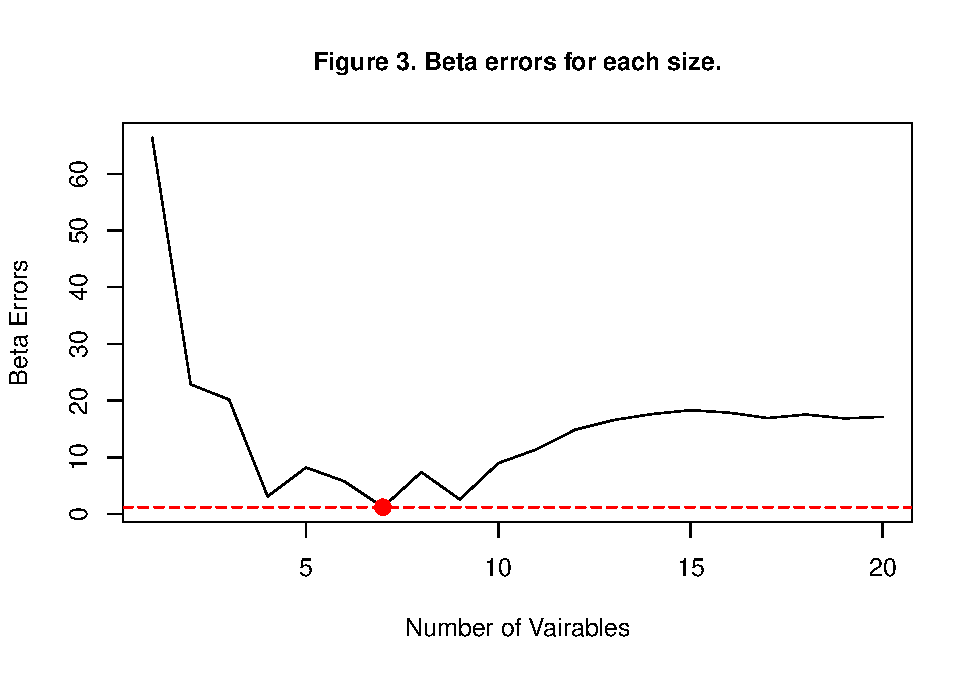
\includegraphics[width=0.5\linewidth,height=0.5\textheight]{Homework_10_Pan_files/figure-latex/unnamed-chunk-11-1}

From the plot we can see that this method selected the 7-predictors
models as the best. However, we do not really know what is the
performance on the testing dataset. We should not rely on this method to
select the best model.

\end{document}
